
\begin{document}



\begin{figure}[t]
\begin{center}
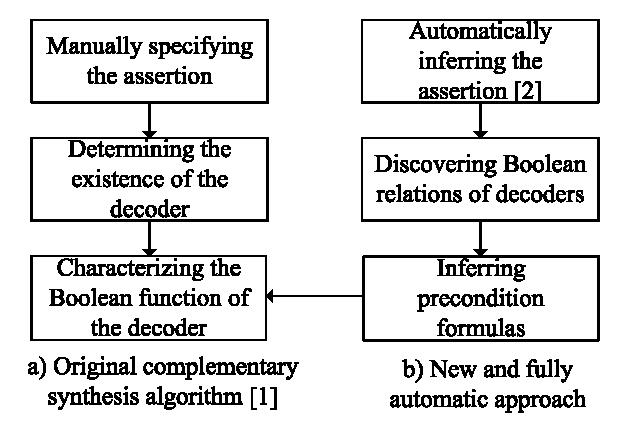
\includegraphics[width=0.35\textwidth]{flow}
\end{center}
\caption{The original and new flows of complementary synthesis}
  \label{flow}
\end{figure}


\begin{figure}[t]
\begin{center}
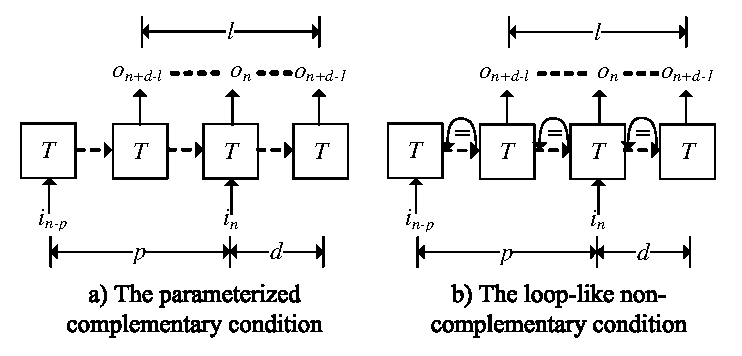
\includegraphics[width=0.5\textwidth]{pcln}
\end{center}
\caption{The parameterized complementary condition and the loop-like non-complementary condition}
  \label{fig_pcln}
\end{figure}



\begin{figure}[t]
\centering
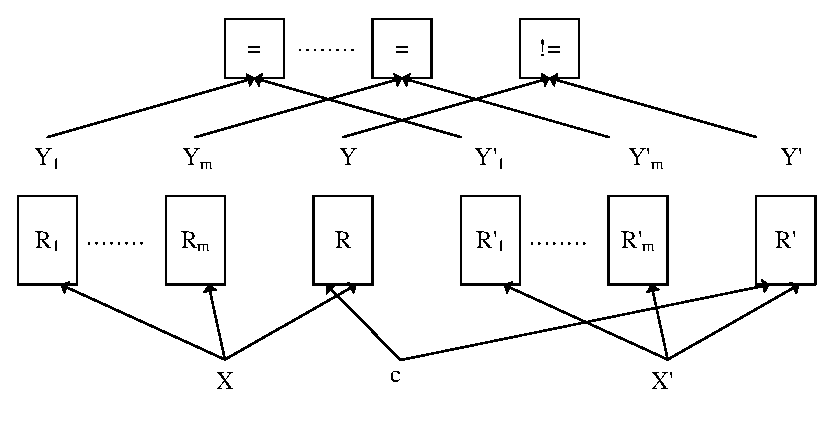
\includegraphics[width=0.45\textwidth]{fdtest}
\caption{The SAT instance that discovers decoders}
\label{fig_fdtest}
\end{figure}

\end{document}


